\chapter{Installation of a '.deb' File}

\YERITHCHAPINTRO{
	\yremphsc{This chapter shows how to
	Install a \debian package management file.}
}


\vspace*{1.05em}


\begin{center}
\captionof{figure}{Gdebi-gtk user graphical interface.}
\yriLabelFORTABLEFigureWITHvspace{-0.49em}{fig:gdebi-gtk-user-graphical-interface}
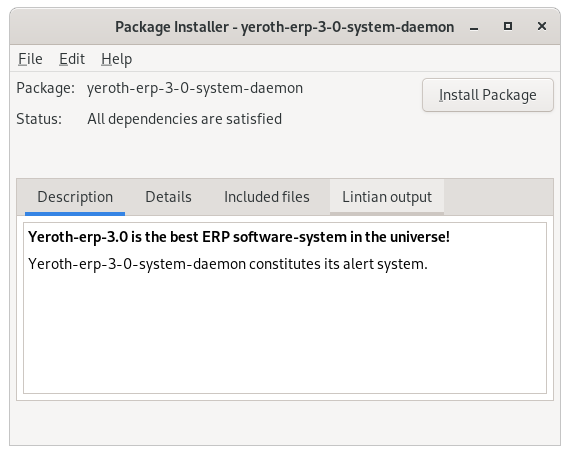
\includegraphics[scale=0.60]{images/YR_GDEBI-GTK.png}
\end{center}


\vspace*{0.95em}


\section{Automated Installation with \gdebigtk and \gdebi}

Program \gdebi and its Graphical User Interface~(GUI)
version \gdebigtk enables one to install a 'deb' file 
without any troubles and~/~or configuration of a \debian 
software packages repository (as for instance in 
file \texttt{''/etc/apt/source.list''}).

\qquad
\yrCOLORDarkred{\gdebi and \gdebigtk have following 
advantage~:~BOTH programs will search all required 
dependent packages--programs and will install them 
automatically for you.}

\qquad
\yrCOLORDarkred{THUS, in this occasion you need to 
configure your \debian software packages repository 
file located at \texttt{''/etc/apt/source.list''}.}



\section{Installation of \gdebigtk and~/~or \gdebi}

\begin{enumerate}[$1.)$]
	\itemsep 0.21em

	\item \yremphsc{Open a ''bash--terminal''}
	
	\item \yremphsc{type following command to install \gdebigtk~:}
		\begin{alltt}
			\rootcommand{apt -y install gdebi-gtk}
		\end{alltt}	
	
	\item \yremphsc{type following command to install \gdebi~:}
		\begin{alltt}
			\rootcommand{apt -y install gdebi}
		\end{alltt}
\end{enumerate} 



\section{Installation with \gdebi}

\begin{enumerate}[$1.)$]
	\itemsep 0.21em

	\item \yremphsc{Open a ''bash--terminal''}
	
	\item \yremphsc{type following command~:}
		\begin{alltt}
			\rootcommand{gdebi -n yerith-erp-9-0-standalone-ENGLISH.deb}
		\end{alltt}
\end{enumerate} 



\section{Installation with \gdebigtk}

\begin{enumerate}[$1.)$]
	\itemsep 0.21em
	
	\item \yremphsc{Open a ''bash--terminal''}
	
	\item \yremphsc{type following command~:}
		\begin{alltt}
			\rootcommand{gdebi-gtk yerith-erp-9-0-standalone-ENGLISH.deb}
		\end{alltt}
		
	\item \yremphsc{press button "Install Package".}
\end{enumerate} 



\newpage




\section{\yremphscBF{\yrCOLORDarkorange{Installation of a Debian Software Repository locally on your Computer}}}

\begin{enumerate}[$1.)$]
	\itemsep 0.21em

	\item 
\end{enumerate} 




\section{\yremphscBF{\yrCOLORDarkred{Installation with \AptDebianPACKAGEManagement Tool}}}

\begin{enumerate}[$1.)$]
	\itemsep 0.21em

	\item \yremphscBF{\yrCOLORDarkorange{Prerequisite~:~You could 
		add all '.deb' into a software \debian repository online.}}
	
	\item \yremphsc{Open a ''bash--terminal''}
	
	\item \yremphsc{type following command~:}
		\begin{alltt}
			\rootcommand{apt -y install yerith-erp-9-0-standalone-configurations-data-ENGLISH}
		\end{alltt}
		
	\item \yremphsc{type following command~:}
		\begin{alltt}
			\rootcommand{apt -y install yerith-erp-9-0-standalone-ENGLISH}
		\end{alltt}

	\item[$\circ$] \yremphscBF{\yrCOLORDarkorange{Or alternatively to the 
		$2$ previous commands, you could issue the following command~:~}}
		{ \scriptsize
		\begin{alltt}
			\rootcommand{apt -y install yerith-erp-9-0-standalone-configurations-data-ENGLISH yerith-erp-9-0-standalone-ENGLISH}
		\end{alltt}
		}
\end{enumerate} 




